\documentclass{article}
\usepackage{graphicx}
\usepackage{float}
\usepackage{geometry}
\usepackage{tcolorbox}
\usepackage{amssymb}
\usepackage{wasysym}
\usepackage{subcaption}
\usepackage{booktabs}
\usepackage{bm}
\usepackage{enumitem}
\usepackage{booktabs}
\usepackage{hyperref}
\usepackage{tabularx} % Required for full-width tables
\usepackage{colortbl} % Required for coloring the table cells
\usepackage{xcolor}   % Required for defining colors
\usepackage{booktabs}



\renewcommand{\labelenumi}{\Roman{enumi}.}
\definecolor{lightgray}{gray}{0.9} % Define lightgray color
\geometry{left=0.8in,right=0.8in,top=0.8in,bottom=1in}

\title{Experiment 2: Experimentation \& Evaluation 2023}
\author{Giorgio Bonetto \& Raffaele Perri}
\date{\today}

\begin{document}
\maketitle
\section*{Abstact}
In this study, we investigate the readability of camelCase versus kebab-case in coding. We conducted experiments with a diverse group of participants, including students and friends. Participants interacted with code snippets containing words in either camelCase or kebab-case. The experiment aimed to assess their speed and accuracy in recognizing and selecting words based on these coding styles. Preliminary results suggest that familiarity with specific coding styles influences reading efficiency. However, the study's limited sample size and participant diversity may affect the generalizability of the findings. 

\section{Introduction}
In the realm of natural language reading, studies have demonstrated that the use of explicit separators between words significantly enhances reading speed—individuals tend to read 20\% faster when such separators are employed. Whether this finding extends to the realm of source code, specifically in the context of composed identifiers, remains an intriguing question. Composed identifiers, featuring more than one word, are commonly used in programming languages, and their readability can impact code comprehension and maintenance.

The focus of this experiment is to investigate whether the observed speedup in reading with explicit separators holds true for composed identifiers in source code. We specifically aim to compare two common styles of composing identifiers: camelCase and kebab-case. CamelCase involves concatenating words together, capitalizing the beginning of each new word (e.g., moveSouth), while kebab-case uses hyphens as separators between words (e.g., move-south).

The motivation behind this study is to shed light on whether the choice of identifier style influences reading efficiency in the context of programming. To achieve this, a controlled experiment has been designed to measure participants' reading speed and accuracy when identifying composed identifiers in both camelCase and kebab-case styles.

This report details the experimental design, methodology, and results of the study, aiming to contribute valuable insights to the ongoing discussion on coding conventions and their impact on code readability. Through a combination of careful experimentation and statistical analysis, we aim to answer the question: Does the choice of identifier style affect the speed and accuracy of code reading?



\begin{tcolorbox}[title=Hypotheses]
    Our experiment is guided by the following hypotheses:
    \begin{itemize}
        \item \textbf{First Hypothesis - Impact of Programming Experience:} The performance in identifying and selecting correct words in code snippets is significantly influenced by the participant's programming experience. We expect that those with more than three years of experience will perform better in terms of accuracy and speed compared to those with less or no experience.

        \item \textbf{Second Hypothesis - Efficiency of Notation Styles:} Participants will complete tasks with kebab-case notation more quickly than those with camelCase. This is due to kebab-case's clear separation of words, which is likely to facilitate quicker recognition and processing, as opposed to camelCase where word boundaries are less distinct.
    \end{itemize}
\end{tcolorbox}




\section{Method}
The method involves conducting a series of experiments where participants interact with code snippets containing words in camelCase or kebab-case. Demographic information is collected before starting the experiments. The participant's choices, correctness, and timing are recorded. The experiment progresses through a set number of trials, and data is submitted for each trial. After completing all experiments, the data is exported to a CSV file. The timing and correctness of responses are key variables of interest.
\subsection{Variables}

\begin{tcolorbox}[title=Independent Variables]

\textbf{Experiment Type (\texttt{currentCase}):}
\begin{itemize}
    \item \textbf{Description:} This variable represents the type of experiment being conducted, whether it's focused on camelCase or kebab-case.
    \item \textbf{Possible Values:} 'camelCase' or 'kebabCase'
\end{itemize}

\textbf{Participant Demographics (\texttt{participantData}):}
\begin{itemize}
    \item \textbf{Description:} Demographic information collected from the participant, including age, gender, programming experience, familiarity with camelCase, and familiarity with kebab-case.
    \item \textbf{Possible Values:} Various based on participant input.
\end{itemize}

\end{tcolorbox}

\begin{tcolorbox}[title=Dependent Variables]

\textbf{Word Selection (\texttt{boxWords}):}
\begin{itemize}
    \item \textbf{Description:} The set of words provided to the participant in each experiment, including the original word and the options in camelCase and kebab-case.
    \item \textbf{Possible Values:} Object containing word information.
\end{itemize}

\textbf{User Interaction and Responses:}
\begin{itemize}
    \item \textbf{Description:} The participant's interaction with the experiment, including clicking on words and the correctness of their choices.
    \item \textbf{Possible Values:} Clicked word, correctness (boolean), time taken.
\end{itemize}

\textbf{Experiment Counter (\texttt{counter}):}
\begin{itemize}
    \item \textbf{Description:} Keeps track of the current experiment number.
    \item \textbf{Possible Values:} Integer from 0 to the total number of experiments.
\end{itemize}

\end{tcolorbox}

\begin{tcolorbox}[title=Control Variables]

\textbf{Total Number of Experiments (\texttt{totalExperiments}):}
\begin{itemize}
    \item \textbf{Description:} Specifies the total number of experiments to be conducted.
    \item \textbf{Fixed Value:} 10 in this case.
\end{itemize}

\textbf{Starting Experiment State (\texttt{statingExperiment}):}
\begin{itemize}
    \item \textbf{Description:} Indicates whether the participant is in the personal information submission phase or the experiment phase.
    \item \textbf{Possible Values:} Boolean (true/false).
\end{itemize}

\end{tcolorbox}

\begin{tcolorbox}[title=Blocking Variables]

\textbf{Time-Related Variables (\texttt{startTime}, \texttt{endTime}, \texttt{timeTaken}):}
\begin{itemize}
    \item \textbf{Description:} Variables related to the timing of participant actions, including the start time, end time, and time taken to respond.
    \item \textbf{Possible Values:} Timestamps and duration in milliseconds.
\end{itemize}

\textbf{Experiment Routing (\texttt{\$router.push}):}
\begin{itemize}
    \item \textbf{Description:} The redirection of the participant to different experiment pages or the end view page.
    \item \textbf{Possible Values:} String (route name or path).
\end{itemize}

\textbf{Attempt Counter (\texttt{attempt}):}
\begin{itemize}
    \item \textbf{Description:} Keeps track of the number of attempts made by the participant in case of an incorrect response before advancing to the next word.
    \item \textbf{Possible Values:} Integer.
\end{itemize}

\end{tcolorbox}

\subsection{Design}
Check off the characteristics of your experimental design:\\

\textbf{Type of Study} (check one):\\
\noindent
\begin{minipage}{0.4\textwidth}
    \fbox{\Square{} \textbf{Observational Study}}
\end{minipage}%
\begin{minipage}{0.4\textwidth}
    \fbox{\bm{\XBox{}} \textbf{Quasi-Experiment}}
\end{minipage}%
\begin{minipage}{0.2\textwidth}
    \fbox{\Square{} \textbf{Experiment}}
\end{minipage}\\\\
The study follows a quasi-experimental design due to practical limitations in manipulating independent variables. Unlike a true experiment with complete control, this design prioritizes real-world conditions.

The experimenter controls the timing of dependent variable measurements but lacks control over participant assignment to different conditions. This compromise ensures a balance between external validity and limitations inherent in coding style familiarity research.

In summary, the quasi-experimental design allows for a nuanced exploration of coding style knowledge across diverse participants, striking a balance between controlled experiments and real-world complexities.
\\


\textbf{Number of Factors} (check one):\\
\noindent
\begin{minipage}{0.4\textwidth}
    \fbox{\Square\ \textbf{Single-Factor Design}}
\end{minipage}%
\begin{minipage}{0.4\textwidth}
    \fbox{\bm{\XBox{}} \textbf{Multi-Factor Design}}
\end{minipage}%
\begin{minipage}{0.0\textwidth}
    \fbox{\Square\ \textbf{Other}}
\end{minipage}\\\\
This experiment employs a Multi-factor Design, encompassing various independent variables to explore participants' responses to code snippets featuring both camelCase and kebab-case formats. The factors under examination include the coding style (randomly assigned as camelCase or kebab-case) and participants' familiarity with each style. These independent variables aim to uncover potential influences on participants' word recognition and selection. The study captures dependent variables, such as participants' responses (correct or incorrect) and the time taken for their selections. The randomized assignment of coding styles enhances the exploration of the interplay between coding style, familiarity, and participant responses within a Multi-factor Design framework:\\
\begin{figure}[H]
    \centering
    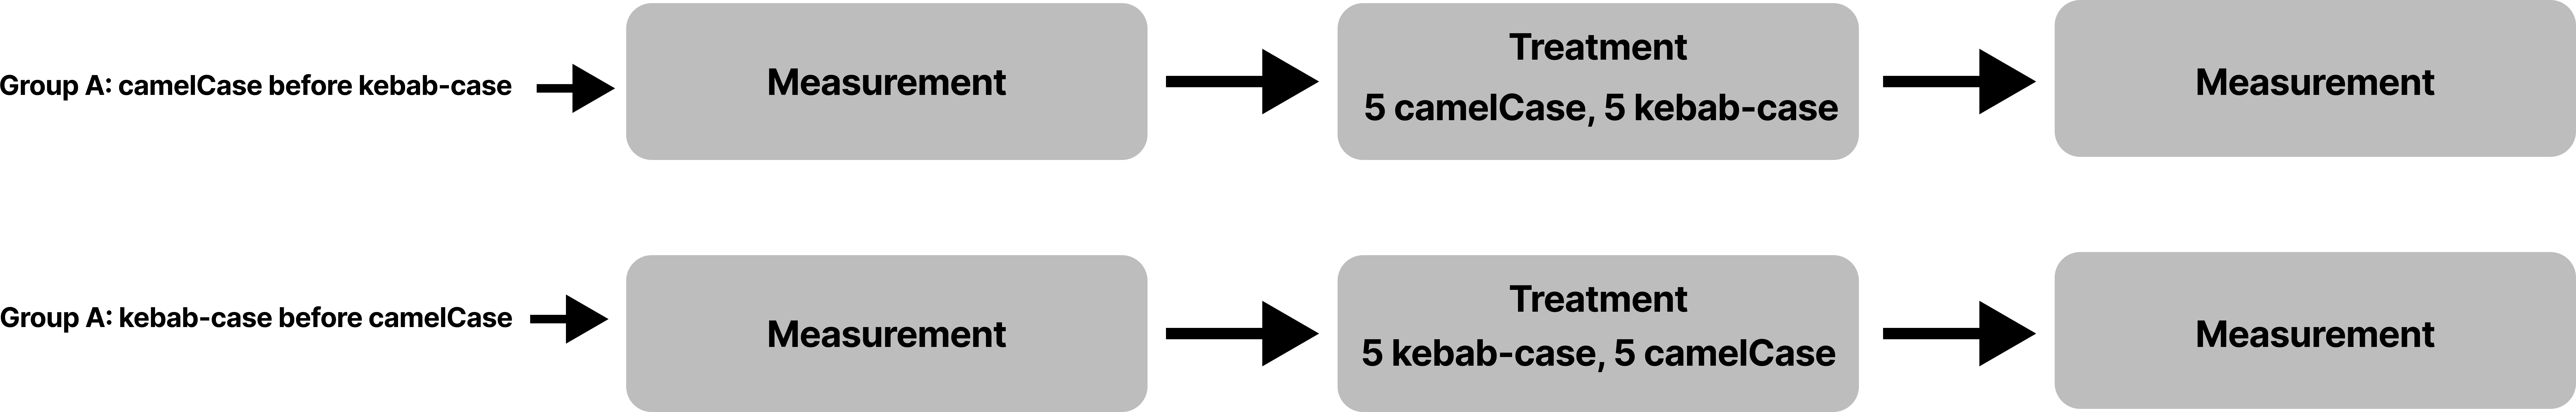
\includegraphics[width=1\textwidth]{graphExperiment2.png}
    \caption{Multi-factor design}
\end{figure}

\subsection{Participants}

The participants in this study encompass a diverse group of individuals, including students, professionals from various fields, and individuals with varying degrees of familiarity with informatics. The recruitment process involved approaching people in person, introducing the study, and inviting them to participate voluntarily.

\subsubsection*{Inclusion Criteria}

Participants were eligible to take part in the study if they:
\begin{itemize}
  \item Expressed willingness to engage in a simple test related to coding conventions.
  \item Represented a broad spectrum of backgrounds, including but not limited to students, non-technical professionals, and individuals with no specific informatics expertise.
\end{itemize}

\subsubsection*{Recruitment Process}

Recruitment was conducted in person, with us (researchers) approaching potential participants in various settings. These settings included educational institutions, public spaces, and community gatherings. The recruitment team provided a brief overview of the study, emphasizing its simplicity and the lack of specific informatics knowledge required.

\subsubsection*{Informed Consent}

Participants were informed about the nature of the study, its objectives, and the procedures involved. They were assured that participation was entirely voluntary and that they could withdraw from the study at any point without consequences. Informed consent was obtained from each participant before engaging in any experimental tasks.

\subsubsection*{Diversity Considerations}

Efforts were made to ensure diversity in the participant pool to capture a broad range of perspectives and experiences. This diversity contributes to the generalizability of findings and allows for a more comprehensive understanding of how individuals with different backgrounds approach coding conventions.

\subsubsection*{Confidentiality and Anonymity}

All collected data were treated with utmost confidentiality. Participants were assigned unique identifiers to protect their anonymity, and personal information was securely stored in compliance with data protection regulations.

\subsection{Apparatus and Materials}


\subsubsection*{Hardware}
The experiment was conducted using a \texttt{Dell Inc Precision 5550} laptop, featuring the following hardware specifications:
\begin{itemize}
  \item \textbf{Processor:} \texttt{Intel® Core™ i7-10850H × 12}
  \item \textbf{RAM:} (Specify the RAM capacity and type)
  \item \textbf{Storage:} (Specify the storage type and capacity)
  \item \textbf{Graphics:} (Specify the graphics card)
  \item \textbf{Display:} (Specify the display specifications)
  \item \textbf{Input Devices:} (Specify any additional input devices used, e.g., mouse, keyboard)
\end{itemize}

\subsubsection*{Software}
The software environment for the experiment was configured as follows:
\begin{itemize}
  \item \textbf{Operating System:} \texttt{Ubuntu 23.04} (64-bit)
  \item \textbf{Kernel Version:} \texttt{Linux 6.2.0-36-generic}
  \item \textbf{Firmware Version:} \texttt{1.24.1}
  \item \textbf{Programming Environment:} \texttt{VisualStudio Code, Intellij IDEA}
\end{itemize}

\subsubsection*{Measurement Tool}
    \begin{itemize}
      \item Utilized the \texttt{performance.now()} function for accurate measurement of execution time.
      \item Employed \texttt{Date.now()} for capturing program execution time.
      \item Used a digital stopwatch to cross-verify the time taken by the program.
    \end{itemize}

\subsubsection*{Experimental Setup}
Participants engaged with the experiment using the provided web application hosted on a local server. The application was accessed through a standard web browser (Google Chrome). The interaction with the experiment was carried out on the \texttt{Dell Inc.Precision 5550} laptop, ensuring a consistent hardware and software environment for all participants.

\subsubsection*{Data Collection Tools}
Data related to participant responses and interactions were collected using the Flask web framework on the server side. Additionally, client-side interactions were captured through the Vue.js framework in the web application. No personally identifiable information was collected, ensuring participant privacy and data confidentiality.

\subsubsection*{Randomization and Counterbalancing}
To minimize potential order effects, the order of presentation for experimental stimuli was randomized for each participant. This randomization was implemented using a custom script within the experimental software.

\subsubsection*{Control Measures}
The experiment was conducted in a controlled environment with minimal external distractions. Participants were provided with standardized instructions to ensure consistency in task execution. The web application interface was designed to be uniform across all sessions.


\subsection{Procedure}

The experiment was conducted in a controlled environment following a standardized procedure. Participants were recruited through in-person interactions, where individuals from a diverse background, including students and those with no prior experience in informatics, were invited to participate in a simple coding style test.

\subsection*{Recruitment}

\begin{itemize}
  \item Participants were approached in person and asked if they would be interested in participating in a coding style test.
  \item The recruitment process involved individuals from various demographics, including students, professionals, and those with diverse interests.
  \item Participants were informed that the test aimed to assess their understanding of coding style conventions in different programming paradigms.
  \item Informed consent was obtained from each participant, emphasizing the voluntary nature of their participation and the confidentiality of their responses.
\end{itemize}

\subsection*{Personal Information Collection}

\begin{itemize}
  \item Participants who expressed interest were directed to a Personal Information View in the web application.
  \item Demographic information, including age, gender, programming experience, and familiarity with coding styles (camelCase and kebab-case), was collected through a structured form.
  \item The personal information collection process was designed to be brief and straightforward, ensuring a seamless transition to the experimental phase.
  \item After providing personal information, participants were guided through the experiment's instructions and purpose.
\end{itemize}

\subsection*{Experiment Instructions}

\begin{itemize}
  \item Participants were introduced to the coding style test, which consisted of 10 code snippets featuring both camelCase and kebab-case examples.
  \item Clear instructions were provided, explaining that each snippet contained clickable words, and participants were required to select the correct word based on coding style conventions.
  \item The experiment emphasized that the task was designed to assess participants' familiarity with coding styles rather than their coding proficiency.
\end{itemize}

\subsection*{Experiment Sessions}

\begin{itemize}
  \item The experiment was divided into two sessions, each featuring 5 code snippets. The order of camelCase and kebab-case snippets was randomized to mitigate order effects.
  \item Participants initiated the experiment by clicking the "Start" button, followed by a brief countdown to ensure readiness.
  \item During each session, participants clicked on words within code snippets, and the web application provided immediate feedback on the correctness of their choices.
  \item Incorrect selections required participants to click on the correct word before proceeding, reinforcing learning through corrective feedback.
\end{itemize}

\subsection*{Data Collection}

\begin{itemize}
  \item Throughout the experiment, participant interactions and responses were recorded, including selected words, response times, and correctness.
  \item After completing the coding style test, participants were directed to a debriefing page, thanking them for their participation and providing information about the study's objectives.
\end{itemize}

\subsection*{Export and Closure}

\begin{itemize}
  \item Participants were informed that their anonymized data would be used for research purposes only.
  \item The experiment concluded with the opportunity for participants to ask questions or seek additional information.
\end{itemize}

The entire procedure aimed to create a standardized and controlled environment for the coding style test while ensuring participant comfort and understanding.


\section{Results}
\subsection{Visual Overview}

After completing the experiment, we analyzed the data collected from various tests. Our primary tool for visualization was the boxen graph, chosen for its exceptional clarity in presenting complex data sets. This graphical method allowed us to easily interpretable visual representations of our findings.

\begin{figure}[H]
    \centering
    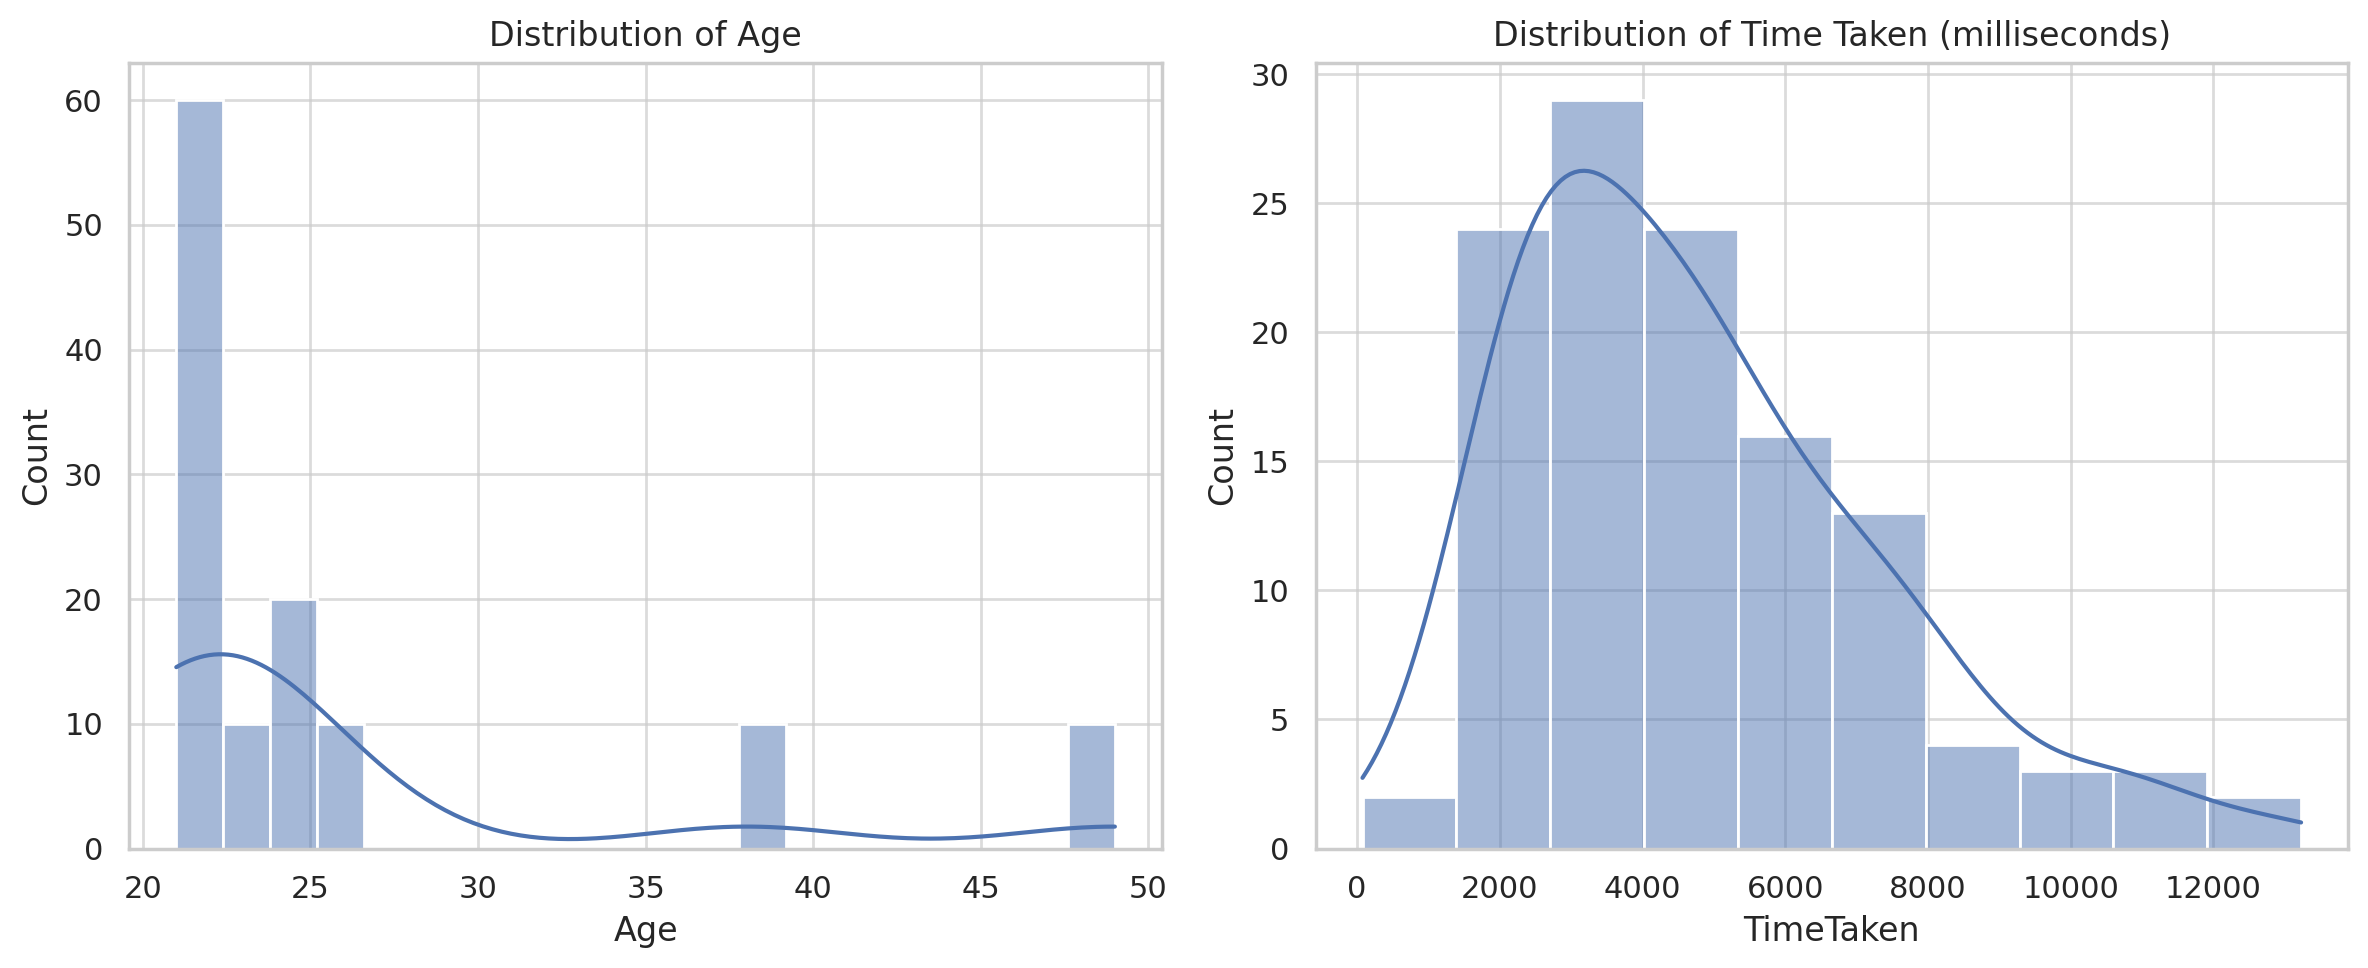
\includegraphics[width=0.8\textwidth]{distribution_age.png}
    \caption{Age and Time Distribution}
\end{figure}

\subsubsection*{Age Distribution of Participants}
The first graph we present focuses on the age distribution of our participants. As illustrated, the majority of our participants are aged between 20 and 25 years. This age concentration aligns with our expectations, considering that most of our test users are students from our university. The graph distinctly shows this age group as the most represented, providing a clear understanding of the demographic makeup of our participant pool.

\subsubsection*{Average Time for Task Completion}
Adjacent to the age distribution graph, we display the average time taken by participants to complete a single task. This graph reveals significant variability in completion times, with some individuals finishing tasks in nearly one second, while others take as long as 12 seconds. Such a wide range suggests that various factors, which we will discuss later, significantly influence task completion time. This variability is a crucial aspect of our analysis, as it underscores the diversity in user interaction with our web application.

\begin{figure}[H]
    \centering
    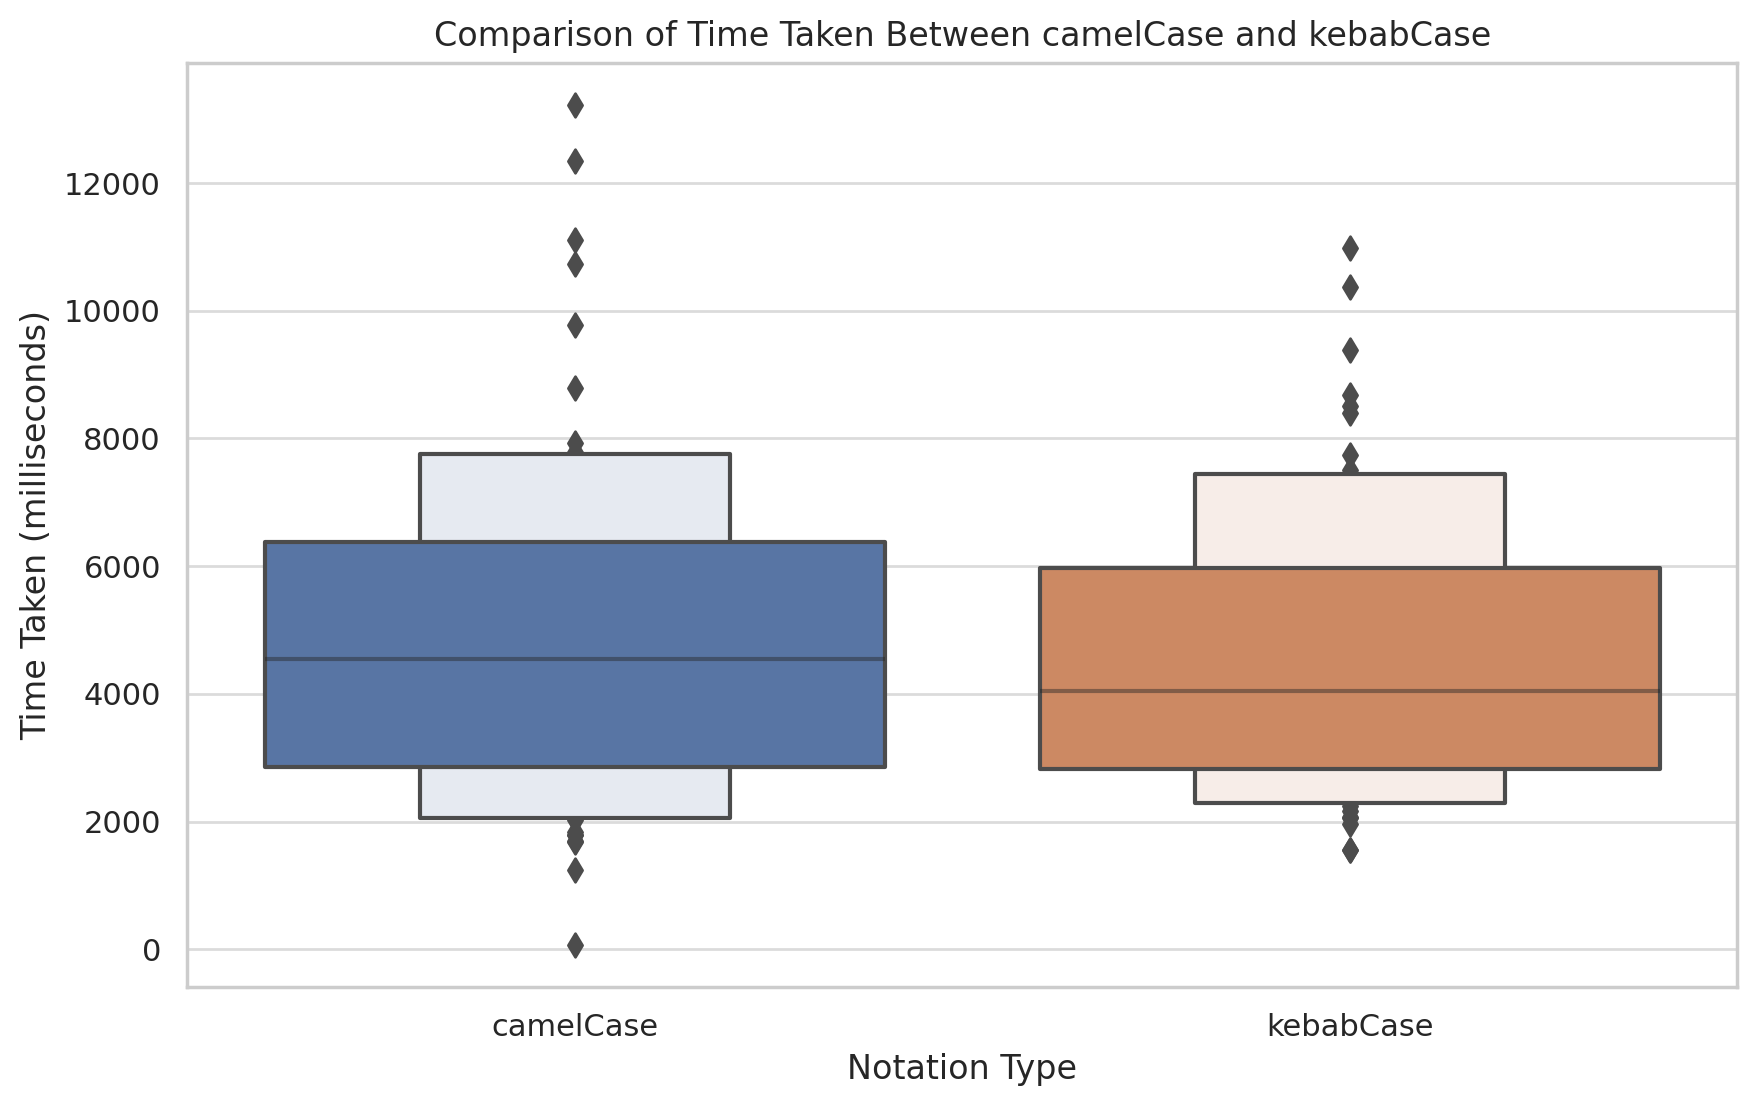
\includegraphics[width=0.8\textwidth]{difference_type.png}
    \caption{Time Between Cmale case and Kebab Case}
\end{figure}

Moreover, this graph is pivotal as it illustrates the difference in time taken between camelCase and kebabCase. Although the distributions appear almost identical, a closer analysis reveals subtle distinctions. Notably, the kebab-case type exhibits a marginally lower average time compared to camelCase. Additionally, the data for kebab-case are more tightly clustered, predominantly within a narrow range of 3 to 6 seconds. In contrast, the camelCase data are more dispersed, resulting in a higher average time.

We want to highlight that the recorded times may be influenced by instances where users had to click more than once, as their initial response was incorrect. This aspect is crucial in understanding the time data, as the need for multiple attempts can significantly impact the total time taken for a task. the number of incorrect answers for camelCase and kebabCase were as follows:

\begin{itemize}
    \item \textbf{Incorrect Responses for camelCase:} There were a total of 13 incorrect responses.
    \item \textbf{Incorrect Responses for kebabCase:} In comparison, kebabCase notation saw a slightly lower number of incorrect responses, totaling 8.
\end{itemize}

This result, as the average time for both camelCase and kebabCase could have been influenced by these incorrect responses.\\


As we progress, it's crucial to consider the distinct methodologies used in Experiment 1 and Experiment 2. Participants in Experiment 1 were first introduced to kebab-case, followed by camelCase. On other hand, Experiment 2 start with camelCase, then proceeded to kebab-case. Notably, these experiments were assigned randomly to participants.

\begin{figure}[H]
    \centering
    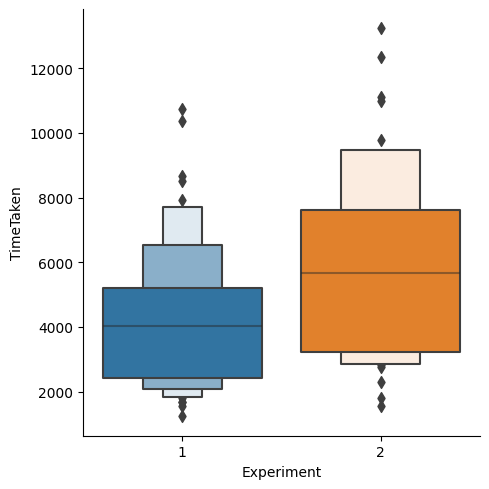
\includegraphics[width=0.6\textwidth]{difference_experiment.png}
    \caption{Different Between Experiment 1 and Experiment 2}
\end{figure}

Our analysis of the data reveals a significant difference between the two experiments. Experiment 1 generally exhibits faster completion times than Experiment 2. This observation suggests that starting with camelCase may present a higher initial challenge to participants, possibly due to its relatively more complex structure or familiarity aspects.

\begin{figure}[H]
    \centering
    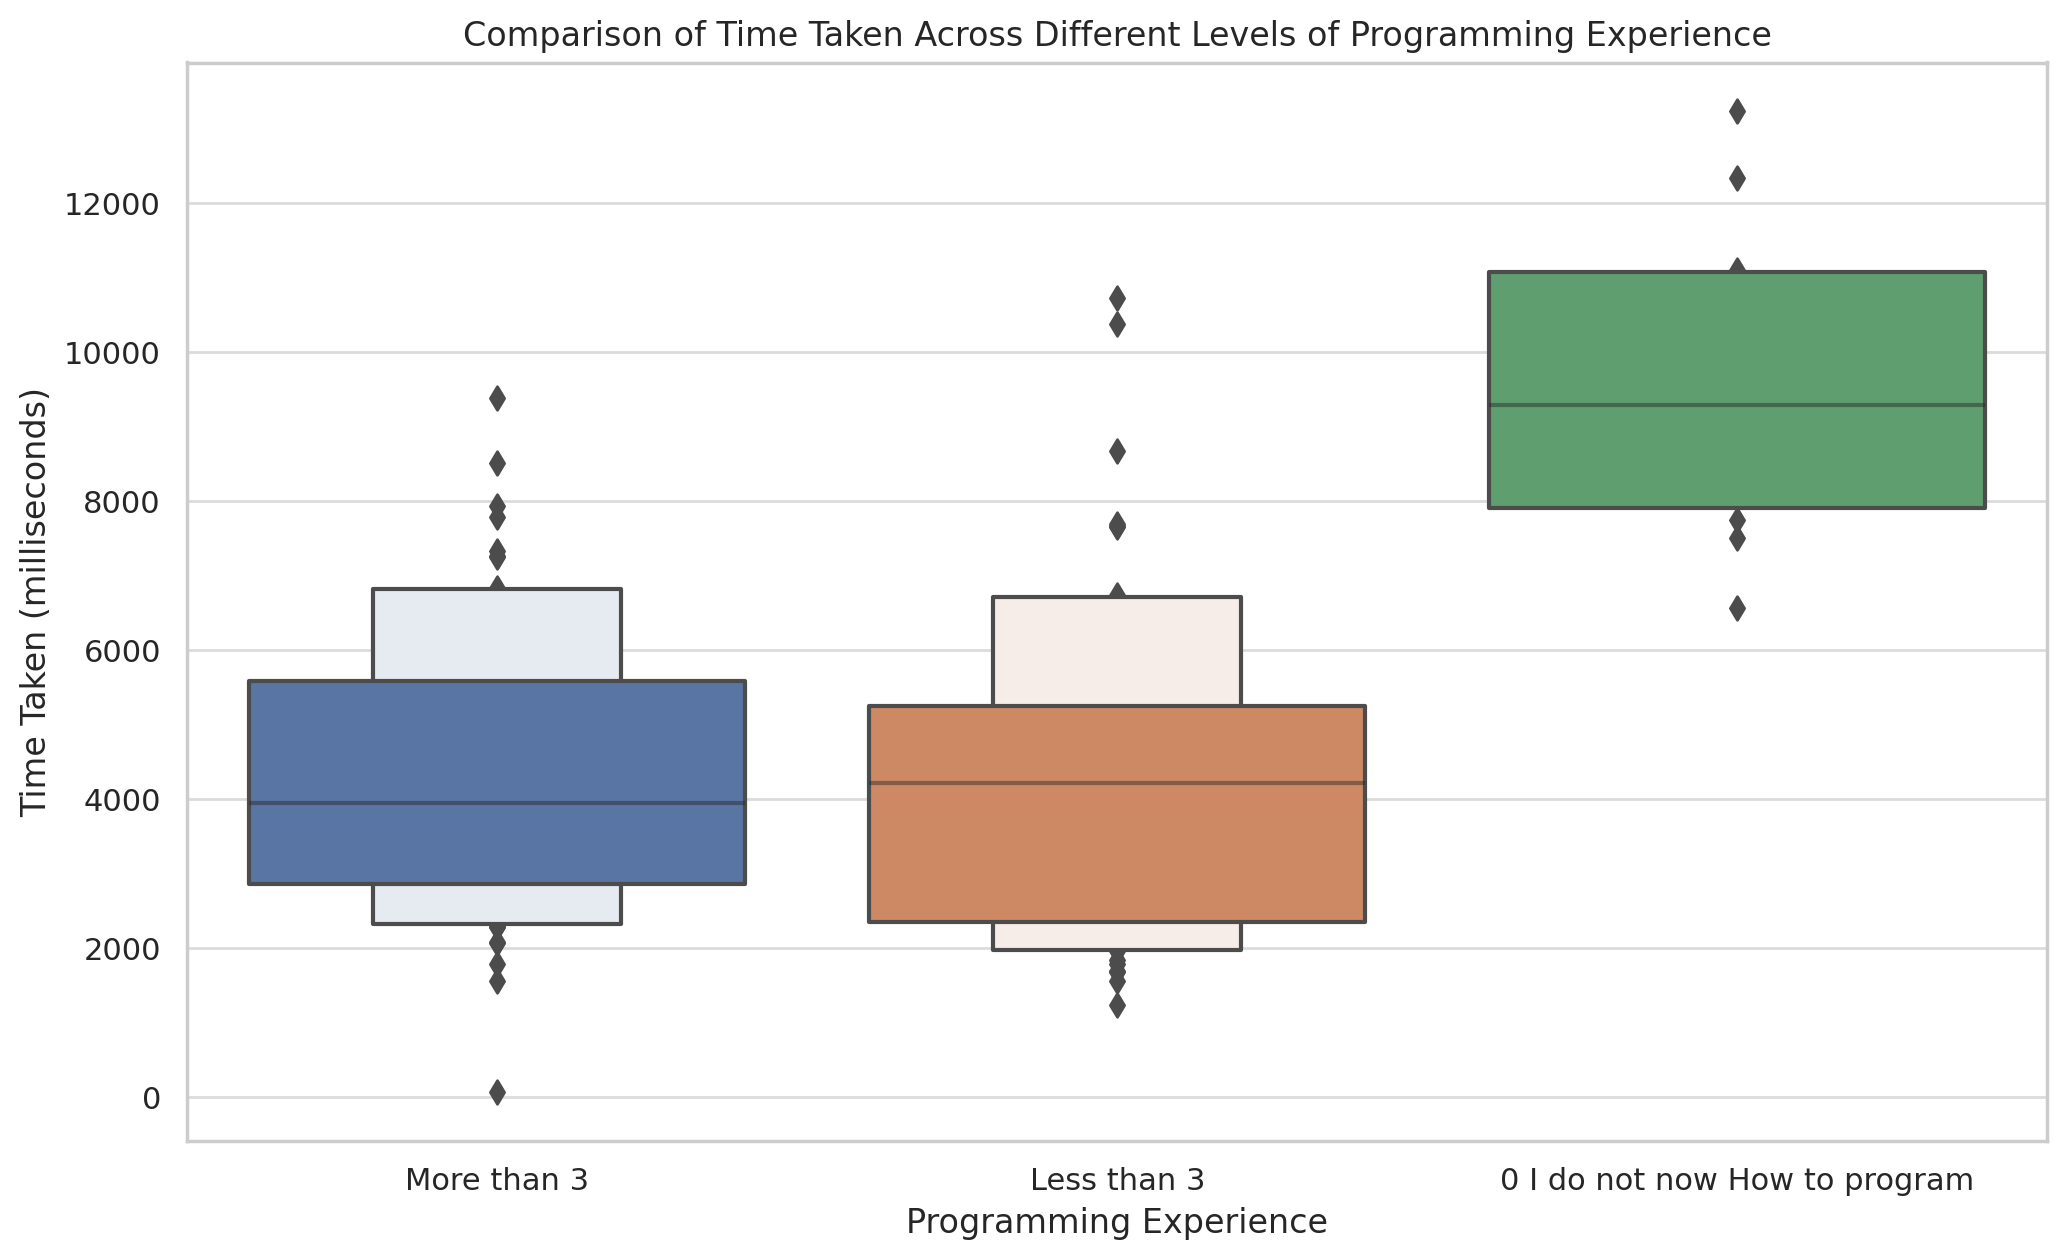
\includegraphics[width=0.6\textwidth]{programming_experience.png}
    \caption{Difference between years of programming experience}
\end{figure}

In our dataset, we further examined the impact of programming experience on task completion times, categorizing participants into three distinct groups: those with no programming experience, those with less than three years of experience, and those with more than three years of experience. The differences in task completion times across these groups were noteworthy. Participants with no programming experience typically took between 8 to 12 seconds to complete a task. Meanwhile, those with less than three years of experience and participants with more than three years of programming experience were much quicker, generally completing tasks within 3 to 6 seconds.



\subsection{Descriptive Statistics}



\begin{table}[h]
	\centering
	\caption{Descriptive Statistics}
	\label{tab:descriptiveStatistics}
	{
		\begin{tabular}{lrrrrrrr}
			\toprule
			 &  & Median & Minimum & Maximum & 25th percentile & 50th percentile & 75th percentile  \\
			\cmidrule[0.4pt]{1-8}
			TimeTaken & camelCase & $4541.700$ & $74.500$ & $13227.600$ & $2854.475$ & $4541.700$ & $6383.400$  \\
			 & kebabCase & $4040.250$ & $1559.500$ & $10977.800$ & $2822.925$ & $4040.250$ & $5970.675$  \\
			\bottomrule
		\end{tabular}
	}
\end{table}

\begin{table}[h]
	\centering
	\caption{Descriptive Statistics}
	\label{tab:descriptiveStatistics}
	{
		\begin{tabular}{lrrr}
			\toprule
			 &  & Mean & Std. Deviation  \\
			\cmidrule[0.4pt]{1-4}
			TimeTaken & camelCase & $4931.910$ & $2815.904$  \\
			 & kebabCase & $4581.095$ & $2289.234$  \\
			\bottomrule
		\end{tabular}
	}
\end{table}

Here we provide a detailed summary of the descriptive statistics for the TimeTaken in both camelCase and kebabCase. These statistics are crucial for understanding the general behavior of the dataset.

\begin{itemize}
\item \textbf{camelCase:}
\begin{itemize}
\item The median time taken is 4541.70 milliseconds, indicating that half of the camelCase tasks were completed in less than this time and the other half took longer.
\item The minimum and maximum times recorded are 74.50 and 13227.60 milliseconds, respectively, showing the range of completion times.
\item The 25th percentile (2854.48 milliseconds) and the 75th percentile (6383.40 milliseconds) mark the lower and upper quartiles, meaning that 25% of the tasks were completed faster than 2854.48 milliseconds and 25% took longer than 6383.40 milliseconds.
\item The mean time taken is 4931.91 milliseconds, with a standard deviation of 2815.90, indicating the average time and the variability around this average.
\item The standard deviation is 2815.90 milliseconds. This relatively high value indicates a wide range around the mean time of 4931.91 milliseconds. In practical terms, it suggests that the time to finish the camelCase test varies greatly among different participants. This variation could be attributed to factors such as individual differences in understanding and applying camelCase notation or different levels of familiarity with the tasks.

\end{itemize}
\item \textbf{kebab-case:}
\begin{itemize}
\item The median time taken is 4040.25 milliseconds, serving as the midpoint of the dataset for kebabCase tasks.
\item The minimum and maximum times are 1559.50 and 10977.80 milliseconds, respectively, indicating the full spread of times.
\item The 25th percentile (2822.93 milliseconds) and the 75th percentile (5970.68 milliseconds) provide insights into the distribution of completion times, showing where the majority of data points lie.
\item The mean time taken is 4581.09 milliseconds, with a standard deviation of 2289.23, reflecting the central tendency and the spread of the data.
\item The standard deviation of 2289.23 milliseconds, slightly lower than that of camelCase. This indicates that test completion times in kebab-case are more clustered around the mean of 4581.09 milliseconds, showing less variability than in camelCase. This could mean that participants found the kebabCase notation more consistent or intuitive, which led to more uniform completion times.

\end{itemize}
\end{itemize}

\subsection{Inferential Statistics}

To test whether the observed differences in time taken between the conditions and groups in our experiment were statistically significant, we used inferential statistics, specifically the t-test for independent samples.


\subsubsection*{T-Test:}
The independent samples t-test is a robust statistical tool used to compare the means of two independent groups. This test is ideal for our analysis because it assesses whether the observed differences in the mean completion times of the two different tests are statistically significant or whether they occurred by chance.\\

The t-test produces two key values: the t-value and the p-value. The t-statistic reflects the magnitude of the difference between the groups with respect to the variability of the data. A higher t-statistic suggests a greater difference between the groups. The p-value indicates the probability of observing such a difference if no difference exists. A p-value less than 0.05 typically suggests that the difference is statistically significant and not just due to random variation.\\

Our t-test, comparing the \textit{TimeTaken} between the different conditions, yielded the following results:
\begin{table}[h]
	\centering
	\caption{Independent Samples T-Test Results}
	\label{tab:independentSamplesTTest}
	{
		\begin{tabular}{lrrr}
			\toprule
			 & T-Statistic & Degrees of Freedom (df) & P-Value  \\
			\cmidrule[0.4pt]{1-4}
			TimeTaken & $0.749$ & $118$ & $0.455$  \\
			\bottomrule
		\end{tabular}
	}
\end{table}

Our p-value of 0.455, which is higher than the conventional threshold of 0.05, suggests that the difference in \textit{TimeTaken} between the groups in our experiment is not statistically significant. This means that the observed differences in time taken could be attributed to chance rather than to a real effect of the conditions tested.

\begin{figure}[H]
    \centering
    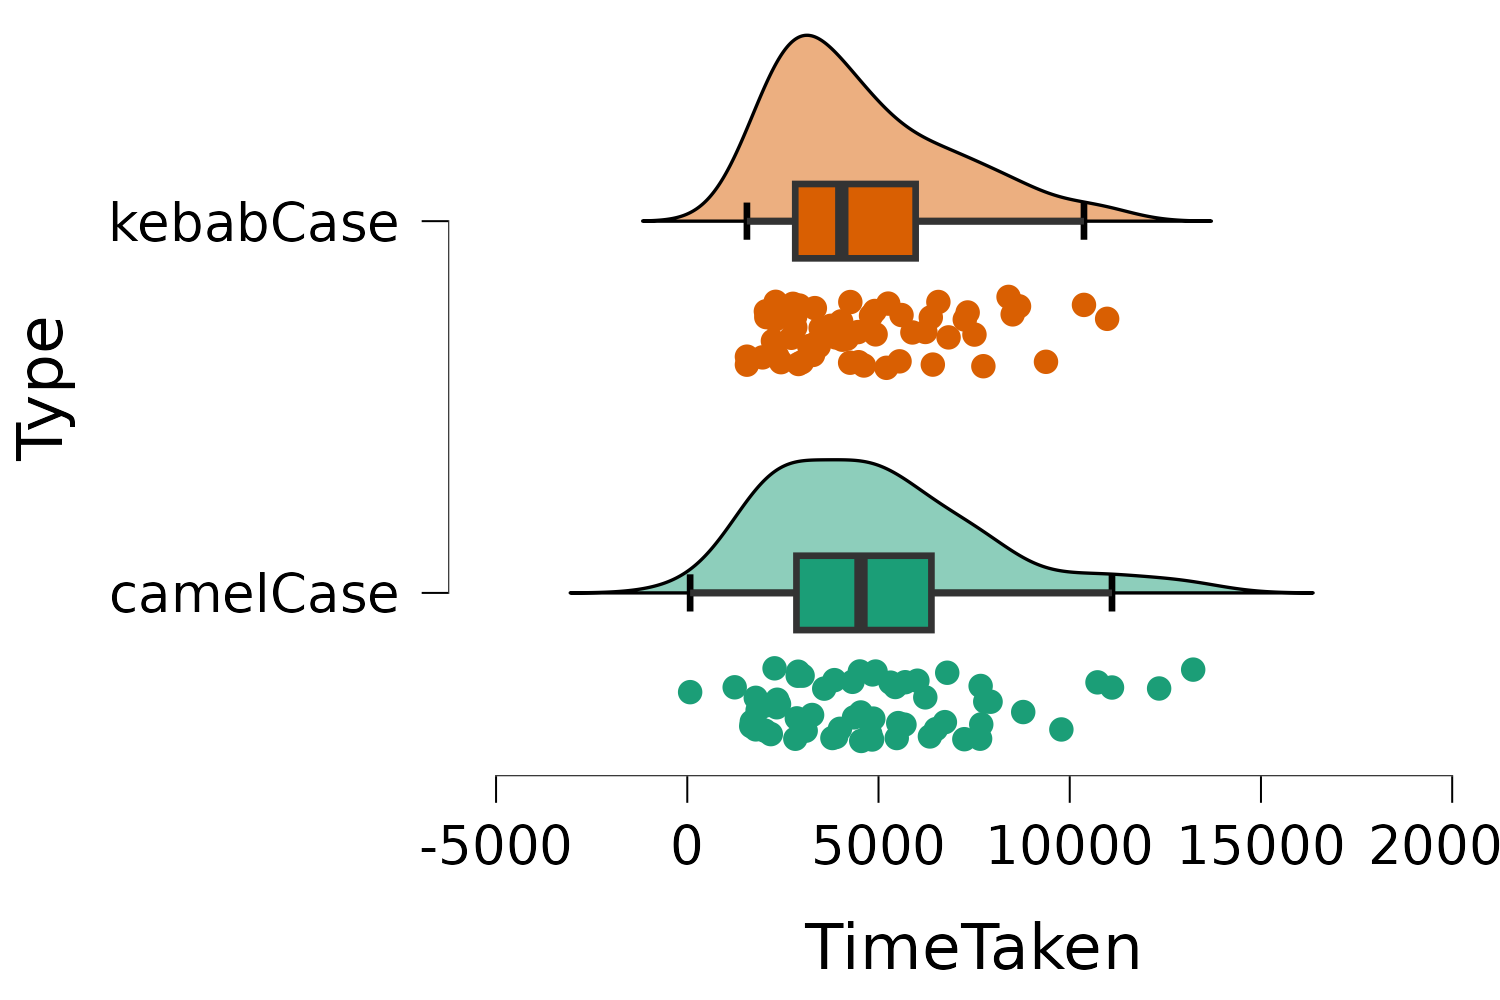
\includegraphics[width=0.4\textwidth]{difference_type_statistics.png}
    \caption{TimeTaken of different type}
\end{figure}

\section{Discussion}
\subsection{Compare Hypothesis to Results}



\label{subsec:compare_hypothesis_results}

In this section, we examine how our experimental findings align with our initial hypotheses, particularly considering the influence of programming experience on task performance.

\paragraph{Revised Hypotheses:}
Our revised hypotheses were as follows:
\begin{enumerate}
    \item \textbf{Impact of Programming Experience on Task Performance:} We hypothesized that the level of programming experience (categorized as no experience, less than three years, and more than three years) would significantly affect participants' ability to correctly and quickly identify and select words in code snippets. Specifically, we anticipated that participants with more than three years of programming experience would outperform those with less or no experience in terms of accuracy and speed.
\end{enumerate}

\paragraph{Assessment of Hypotheses:}
\begin{itemize}
    \item \textbf{Programming Experience and Task Performance:} The results from our experiment supported this hypothesis. Participants with more than three years of programming experience consistently showed quicker and more accurate task completion. Those with no programming experience typically took longer, between 8 to 12 seconds, to complete a task. In contrast, participants with more than three years of experience could complete tasks within 3 to 6 seconds, indicating a clear correlation between programming experience and task performance efficiency.
    
    \item \textbf{Comparative Analysis of Notation Styles:} While our initial hypothesis also considered the impact of notation style (camelCase and kebab-case), the results did not reveal a significant difference in performance based on these styles alone. This suggests that the programming experience of participants was a more decisive factor in their task performance than the specific coding notation used.
\end{itemize}

\paragraph{Reflection on Findings:}
The alignment of the experimental results with our hypothesis regarding programming experience underscores the importance of familiarity and proficiency in programming. It suggests that experience in coding not only improves accuracy but also efficiency in processing and responding to coding-related tasks. The lack of significant difference attributed to notation style, however, indicates that the efficiency of processing different coding styles may be more uniform across experienced programmers, overshadowing the nuances between camelCase and kebab-case.


Moreover the results of the t-test conducted in our study show, the statistical analysis did not provide sufficient evidence to reject the null hypothesis. This result suggests that there is no significant difference in completion times between groups in the conditions tested in our experiment.

These results are of considerable importance as they contribute to the understanding of the impact of the conditions tested on task completion times. 

\subsection{Limitations and Threats to Validity}
This study, while providing insights into the readability of camelCase and kebab-case, has certain limitations that must be acknowledged for a comprehensive understanding.

\begin{itemize}
  \item \textbf{Participant Diversity:} The participants predominantly comprised university students with a background in informatics. Future studies could benefit from a more diverse demographic, including individuals from varied professional and educational backgrounds, to enhance the generalizability of the findings.

  \item \textbf{Word Selection in Code Snippets:} The random selection of words for code snippets may have introduced varying levels of difficulty, potentially affecting task completion times. A more controlled and balanced selection of words in future experiments could yield more accurate comparative results.

  \item \textbf{Sample Size and Repetition:} The sample size and the number of trials per participant in this study may not suffice to draw definitive conclusions. Increasing these factors could lead to more robust and reliable results.
\end{itemize}

These factors should be considered in future research to enhance the reliability and applicability of the results in the broader context of code readability and efficiency.

\subsection{Conclusions}

In this experiment, we aimed to investigate the impact of coding style familiarity on participants' accuracy and speed in identifying and selecting words in code snippets. Our primary focus was on two commonly used coding styles: camelCase and kebab-case. Through a multi-factor design, we explored the interplay between coding style, familiarity, and participant responses.

Our hypothesis suggested that participants familiar with both camelCase and kebab-case would demonstrate higher accuracy in their selections. However, the results of our experiment did not support this hypothesis. The differences in time taken between camelCase and kebab-case were not found to be statistically significant, indicating that coding style familiarity might not have a significant impact on task completion time in our experimental setting.

While our findings challenge the initial hypothesis, they provide valuable insights into the complexity of factors influencing code reading. The observed variability in completion times across participants, as well as the influence of the experiment order on task difficulty, highlights the nuanced nature of coding style comprehension.

It's essential to acknowledge the limitations of our study, including the specific context of the experiment and the diversity of participant backgrounds. The quasi-experimental design, although practical, may limit the generalizability of our findings to broader programming contexts.

In conclusion, our experiment contributes to the ongoing discussion on coding conventions and their influence on code readability. Future research could explore additional factors, such as individual cognitive styles and task complexity, to provide a more comprehensive understanding of code reading processes. Despite the challenges and unexpected results, this study emphasizes the importance of considering various elements in designing experiments that capture the intricacies of programming-related tasks.


\section{Appendix}
\subsection*{A. Materials}
\textbf{Book: } \textit{How to Design and Report Experiments} by Andy Field and Graham J Hole\\
\textbf{Software: } \textit{Jasp, Google Colab} for statistical analysis, \textit{Visual Studio Code}, \textit{Figma} for multi-factor design\\
\textbf{Programming Language: } \textit{Python} for implementation of word randomization and creation,
\textit{Vue.js, Javascript} for the website creation \\
\textbf{Machine: } \textit {Dell Inc. Precision 5550 }

\subsection{Reproduction Package}

Before, during, and after the experiment you collected all kinds of data. Don't ever throw such data away! Any plots, tables, summaries, and statistics provided in this report should be recreatable from the raw data you have.

If you only collected a small amount of data, put it in this Appendix right here.

If you collected data in forms that are better kept in separate files, then zip up those files, and submit them as a "reproduction package" supporting this report.


\subsection*{{Github repo: (\url{https://github.com/Bonett0/experiment-02})}}




\end{document}
